\item Un experimentador está estudiando los efectos de la temperatura, la presión y el tipo de catalizador en la producción de cierta reacción química. Se consideran para las experiencias tres temperaturas diferentes, cuatro presiones distintas y cinco catalizadores diferentes. Si cualquier experimento particular implica utilizar una temperatura, una presión y un catalizador:
    \begin{enumerate}
        \item ¿Cuántos experimentos distintos son posibles realizar?\e\\
            Hay 3 temperaturas, 4 presiones y 5 catalizadores. Entonces,\[\#experimentos=3\cdot4\cdot5=60\]
            Sean \begin{align*}
                T_i&=\text{"Temperatura $i$"},i=1,2,3\\
                P_i&=\text{"Presión $i$"}, i=1,2,3,4\\
                C_i&=\text{"Catalizador $i$"},i=1,2,3,4,5
            \end{align*}
            las combinaciones calculadas previamente calculadas se pueden visualizar en el siguiente diagrama de árbol
            \begin{center}
                \tikzstyle{level 1}=[level distance=30mm, sibling distance=55.5mm]
                \tikzstyle{level 2}=[level distance=30mm, sibling distance=14mm]
                \tikzstyle{level 3}=[level distance=30mm,sibling distance=2.5mm]
                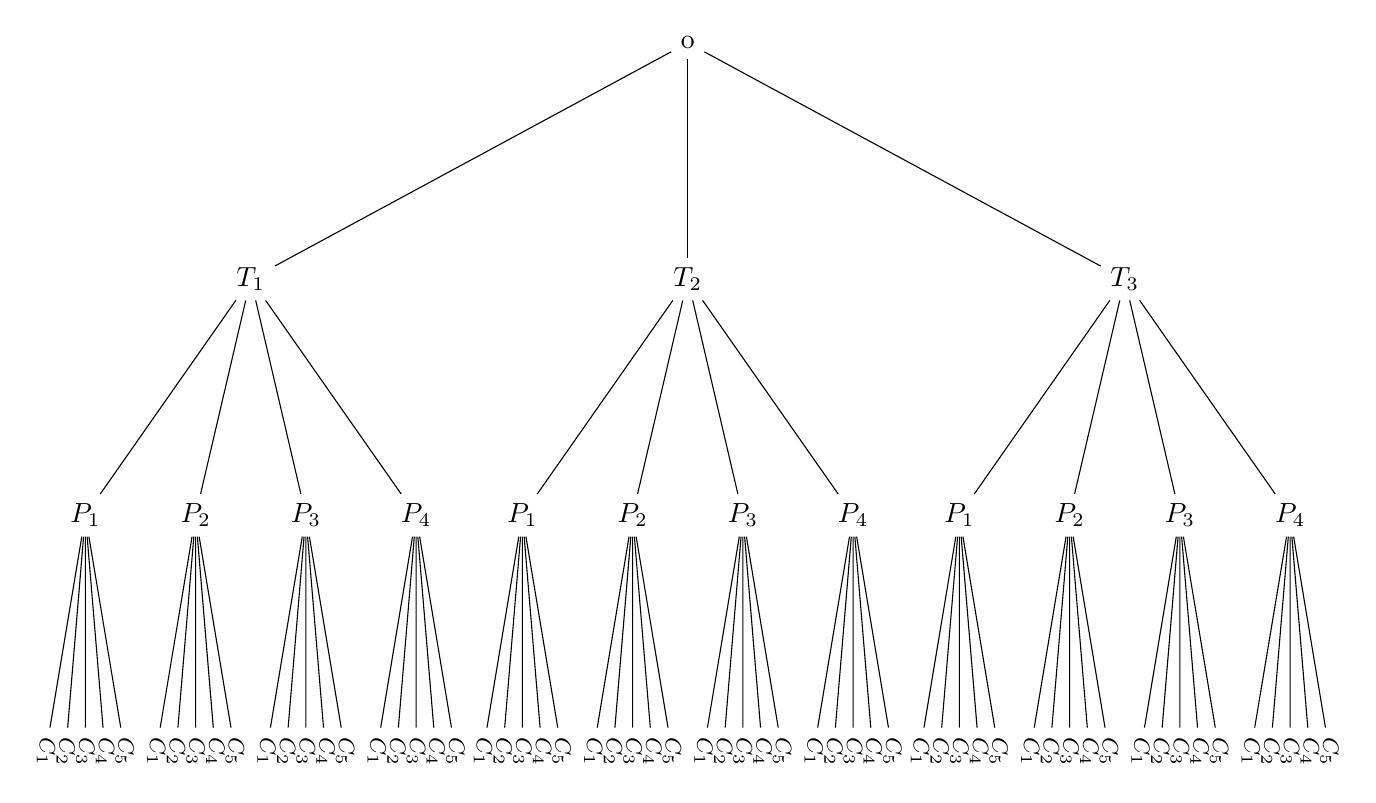
\begin{tikzpicture}[grow=down]
                    \begin{scope}[yshift=0]
                    \node {o}
                        child{
                            node {$T_1$}
                                child{
                                    node {$P_1$}
                                        child{node{\rotatebox{270}{\footnotesize{$C_1$}}}}
                                        child{node{\rotatebox{270}{\footnotesize{$C_2$}}}}
                                        child{node{\rotatebox{270}{\footnotesize{$C_3$}}}}
                                        child{node{\rotatebox{270}{\footnotesize{$C_4$}}}}
                                        child{node{\rotatebox{270}{\footnotesize{$C_5$}}}}
                                }
                                child {
                                    node{$P_2$}
                                        child{node{\rotatebox{270}{\footnotesize{$C_1$}}}}
                                        child{node{\rotatebox{270}{\footnotesize{$C_2$}}}}
                                        child{node{\rotatebox{270}{\footnotesize{$C_3$}}}}
                                        child{node{\rotatebox{270}{\footnotesize{$C_4$}}}}
                                        child{node{\rotatebox{270}{\footnotesize{$C_5$}}}}
                                }
                                child {
                                    node{$P_3$}
                                        child{node{\rotatebox{270}{\footnotesize{$C_1$}}}}
                                        child{node{\rotatebox{270}{\footnotesize{$C_2$}}}}
                                        child{node{\rotatebox{270}{\footnotesize{$C_3$}}}}
                                        child{node{\rotatebox{270}{\footnotesize{$C_4$}}}}
                                        child{node{\rotatebox{270}{\footnotesize{$C_5$}}}}
                                }
                                child {
                                    node{$P_4$}
                                        child{node{\rotatebox{270}{\footnotesize{$C_1$}}}}
                                        child{node{\rotatebox{270}{\footnotesize{$C_2$}}}}
                                        child{node{\rotatebox{270}{\footnotesize{$C_3$}}}}
                                        child{node{\rotatebox{270}{\footnotesize{$C_4$}}}}
                                        child{node{\rotatebox{270}{\footnotesize{$C_5$}}}}
                                }
                        }
                        child{
                            node {$T_2$}
                                child{
                                    node {$P_1$}
                                        child{node{\rotatebox{270}{\footnotesize{$C_1$}}}}
                                        child{node{\rotatebox{270}{\footnotesize{$C_2$}}}}
                                        child{node{\rotatebox{270}{\footnotesize{$C_3$}}}}
                                        child{node{\rotatebox{270}{\footnotesize{$C_4$}}}}
                                        child{node{\rotatebox{270}{\footnotesize{$C_5$}}}}
                                }
                                child {
                                    node{$P_2$}
                                        child{node{\rotatebox{270}{\footnotesize{$C_1$}}}}
                                        child{node{\rotatebox{270}{\footnotesize{$C_2$}}}}
                                        child{node{\rotatebox{270}{\footnotesize{$C_3$}}}}
                                        child{node{\rotatebox{270}{\footnotesize{$C_4$}}}}
                                        child{node{\rotatebox{270}{\footnotesize{$C_5$}}}}
                                }
                                child {
                                    node{$P_3$}
                                        child{node{\rotatebox{270}{\footnotesize{$C_1$}}}}
                                        child{node{\rotatebox{270}{\footnotesize{$C_2$}}}}
                                        child{node{\rotatebox{270}{\footnotesize{$C_3$}}}}
                                        child{node{\rotatebox{270}{\footnotesize{$C_4$}}}}
                                        child{node{\rotatebox{270}{\footnotesize{$C_5$}}}}
                                }
                                child {
                                    node{$P_4$}
                                        child{node{\rotatebox{270}{\footnotesize{$C_1$}}}}
                                        child{node{\rotatebox{270}{\footnotesize{$C_2$}}}}
                                        child{node{\rotatebox{270}{\footnotesize{$C_3$}}}}
                                        child{node{\rotatebox{270}{\footnotesize{$C_4$}}}}
                                        child{node{\rotatebox{270}{\footnotesize{$C_5$}}}}
                                }
                        }
                        child{
                            node {$T_3$}
                                child{
                                    node {$P_1$}
                                        child{node{\rotatebox{270}{\footnotesize{$C_1$}}}}
                                        child{node{\rotatebox{270}{\footnotesize{$C_2$}}}}
                                        child{node{\rotatebox{270}{\footnotesize{$C_3$}}}}
                                        child{node{\rotatebox{270}{\footnotesize{$C_4$}}}}
                                        child{node{\rotatebox{270}{\footnotesize{$C_5$}}}}
                                }
                                child {
                                    node{$P_2$}
                                        child{node{\rotatebox{270}{\footnotesize{$C_1$}}}}
                                        child{node{\rotatebox{270}{\footnotesize{$C_2$}}}}
                                        child{node{\rotatebox{270}{\footnotesize{$C_3$}}}}
                                        child{node{\rotatebox{270}{\footnotesize{$C_4$}}}}
                                        child{node{\rotatebox{270}{\footnotesize{$C_5$}}}}
                                }
                                child {
                                    node{$P_3$}
                                        child{node{\rotatebox{270}{\footnotesize{$C_1$}}}}
                                        child{node{\rotatebox{270}{\footnotesize{$C_2$}}}}
                                        child{node{\rotatebox{270}{\footnotesize{$C_3$}}}}
                                        child{node{\rotatebox{270}{\footnotesize{$C_4$}}}}
                                        child{node{\rotatebox{270}{\footnotesize{$C_5$}}}}
                                }
                                child {
                                    node{$P_4$}
                                        child{node{\rotatebox{270}{\footnotesize{$C_1$}}}}
                                        child{node{\rotatebox{270}{\footnotesize{$C_2$}}}}
                                        child{node{\rotatebox{270}{\footnotesize{$C_3$}}}}
                                        child{node{\rotatebox{270}{\footnotesize{$C_4$}}}}
                                        child{node{\rotatebox{270}{\footnotesize{$C_5$}}}}
                                }
                        };
                    \end{scope}
                \end{tikzpicture}
            \end{center}
        \item ¿Cuántos experimentos distintos existen que impliquen el uso de la temperatura más baja y las dos presiones más bajas?\e\\
            Hay una única temperatura más baja, y hay una restricción a 2 presiones en particular, por ende\[\#experimentos^\prime=1\cdot2\cdot5=10\]
            Con el diagrama de árbol, podemos establecer que la temperatura más baja es $T_1$ y que las presiones más bajas son $P_1$ y $P_2$, con lo cual, se reprenta con naranja cada rama en la que están involucradas estas condiciones
            \begin{center}
                \tikzstyle{level 1}=[level distance=30mm, sibling distance=55.5mm]
                \tikzstyle{level 2}=[level distance=30mm, sibling distance=14mm]
                \tikzstyle{level 3}=[level distance=30mm,sibling distance=2.5mm]
                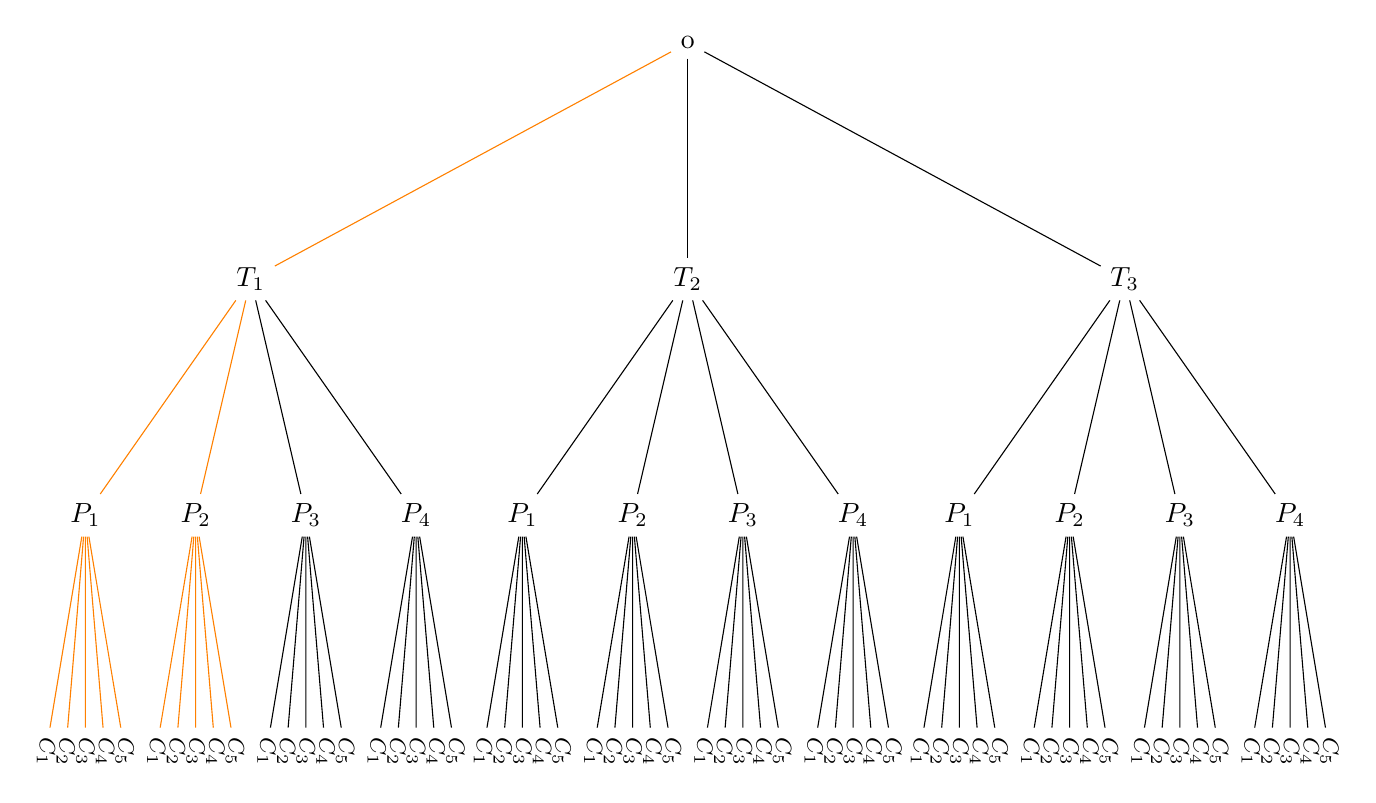
\begin{tikzpicture}[grow=down]
                    \begin{scope}[yshift=0]
                    \node {o}
                        child {
                            node {$T_1$} edge from parent [orange]
                                child{
                                    node [black] {$P_1$} edge from parent [orange]
                                        child{node [black] {\rotatebox{270}{\footnotesize{$C_1$}}}}
                                        child{node [black] {\rotatebox{270}{\footnotesize{$C_2$}}}}
                                        child{node [black] {\rotatebox{270}{\footnotesize{$C_3$}}}}
                                        child{node [black] {\rotatebox{270}{\footnotesize{$C_4$}}}}
                                        child{node [black] {\rotatebox{270}{\footnotesize{$C_5$}}}}
                                }
                                child {
                                    node [black] {$P_2$} edge from parent [orange]
                                        child{node [black] {\rotatebox{270}{\footnotesize{$C_1$}}}}
                                        child{node [black] {\rotatebox{270}{\footnotesize{$C_2$}}}}
                                        child{node [black] {\rotatebox{270}{\footnotesize{$C_3$}}}}
                                        child{node [black] {\rotatebox{270}{\footnotesize{$C_4$}}}}
                                        child{node [black] {\rotatebox{270}{\footnotesize{$C_5$}}}}
                                }
                                child {
                                    node [black] {$P_3$} edge from parent [black]
                                        child{node{\rotatebox{270}{\footnotesize{$C_1$}}}}
                                        child{node{\rotatebox{270}{\footnotesize{$C_2$}}}}
                                        child{node{\rotatebox{270}{\footnotesize{$C_3$}}}}
                                        child{node{\rotatebox{270}{\footnotesize{$C_4$}}}}
                                        child{node{\rotatebox{270}{\footnotesize{$C_5$}}}}
                                }
                                child {
                                    node [black] {$P_4$} edge from parent [black]
                                        child{node{\rotatebox{270}{\footnotesize{$C_1$}}}}
                                        child{node{\rotatebox{270}{\footnotesize{$C_2$}}}}
                                        child{node{\rotatebox{270}{\footnotesize{$C_3$}}}}
                                        child{node{\rotatebox{270}{\footnotesize{$C_4$}}}}
                                        child{node{\rotatebox{270}{\footnotesize{$C_5$}}}}
                                }
                        }
                        child{
                            node {$T_2$}
                                child{
                                    node {$P_1$}
                                        child{node{\rotatebox{270}{\footnotesize{$C_1$}}}}
                                        child{node{\rotatebox{270}{\footnotesize{$C_2$}}}}
                                        child{node{\rotatebox{270}{\footnotesize{$C_3$}}}}
                                        child{node{\rotatebox{270}{\footnotesize{$C_4$}}}}
                                        child{node{\rotatebox{270}{\footnotesize{$C_5$}}}}
                                }
                                child {
                                    node{$P_2$}
                                        child{node{\rotatebox{270}{\footnotesize{$C_1$}}}}
                                        child{node{\rotatebox{270}{\footnotesize{$C_2$}}}}
                                        child{node{\rotatebox{270}{\footnotesize{$C_3$}}}}
                                        child{node{\rotatebox{270}{\footnotesize{$C_4$}}}}
                                        child{node{\rotatebox{270}{\footnotesize{$C_5$}}}}
                                }
                                child {
                                    node{$P_3$}
                                        child{node{\rotatebox{270}{\footnotesize{$C_1$}}}}
                                        child{node{\rotatebox{270}{\footnotesize{$C_2$}}}}
                                        child{node{\rotatebox{270}{\footnotesize{$C_3$}}}}
                                        child{node{\rotatebox{270}{\footnotesize{$C_4$}}}}
                                        child{node{\rotatebox{270}{\footnotesize{$C_5$}}}}
                                }
                                child {
                                    node{$P_4$}
                                        child{node{\rotatebox{270}{\footnotesize{$C_1$}}}}
                                        child{node{\rotatebox{270}{\footnotesize{$C_2$}}}}
                                        child{node{\rotatebox{270}{\footnotesize{$C_3$}}}}
                                        child{node{\rotatebox{270}{\footnotesize{$C_4$}}}}
                                        child{node{\rotatebox{270}{\footnotesize{$C_5$}}}}
                                }
                        }
                        child{
                            node {$T_3$}
                                child{
                                    node {$P_1$}
                                        child{node{\rotatebox{270}{\footnotesize{$C_1$}}}}
                                        child{node{\rotatebox{270}{\footnotesize{$C_2$}}}}
                                        child{node{\rotatebox{270}{\footnotesize{$C_3$}}}}
                                        child{node{\rotatebox{270}{\footnotesize{$C_4$}}}}
                                        child{node{\rotatebox{270}{\footnotesize{$C_5$}}}}
                                }
                                child {
                                    node{$P_2$}
                                        child{node{\rotatebox{270}{\footnotesize{$C_1$}}}}
                                        child{node{\rotatebox{270}{\footnotesize{$C_2$}}}}
                                        child{node{\rotatebox{270}{\footnotesize{$C_3$}}}}
                                        child{node{\rotatebox{270}{\footnotesize{$C_4$}}}}
                                        child{node{\rotatebox{270}{\footnotesize{$C_5$}}}}
                                }
                                child {
                                    node{$P_3$}
                                        child{node{\rotatebox{270}{\footnotesize{$C_1$}}}}
                                        child{node{\rotatebox{270}{\footnotesize{$C_2$}}}}
                                        child{node{\rotatebox{270}{\footnotesize{$C_3$}}}}
                                        child{node{\rotatebox{270}{\footnotesize{$C_4$}}}}
                                        child{node{\rotatebox{270}{\footnotesize{$C_5$}}}}
                                }
                                child {
                                    node{$P_4$}
                                        child{node{\rotatebox{270}{\footnotesize{$C_1$}}}}
                                        child{node{\rotatebox{270}{\footnotesize{$C_2$}}}}
                                        child{node{\rotatebox{270}{\footnotesize{$C_3$}}}}
                                        child{node{\rotatebox{270}{\footnotesize{$C_4$}}}}
                                        child{node{\rotatebox{270}{\footnotesize{$C_5$}}}}
                                }
                        };
                    \end{scope}
                \end{tikzpicture}
            \end{center}
        \item Suponga que se tiene que realizar cinco experimentos diferentes el primer día de experimentación y los experimentos se realizar al azar. ¿Cuál es la probabilidad de que se utilice un catalizador diferente en cada experimento?\e\\
            Los casos favorables: el primer experimento no tiene restricción, entonces hay 5 opciones. Para el segundo, no puedo usar el catalizador del primero, así que hay 4 opciones, por los mismos motivos, para el tercero hay 3, para el cuarto 2 y para el quinto 1. Casos totales: no hay restricción alguna en los experimentos, así que siendo $A=$"no se repite el catalizador", se tiene que\[P(A)=\frac{\text{casos favorables}}{\text{casos totales}}=\frac{5!}{5^5}\]
    \end{enumerate}